\section{System Model}
\label{sec:system model}
\begin{figure}[t]
	\centering
   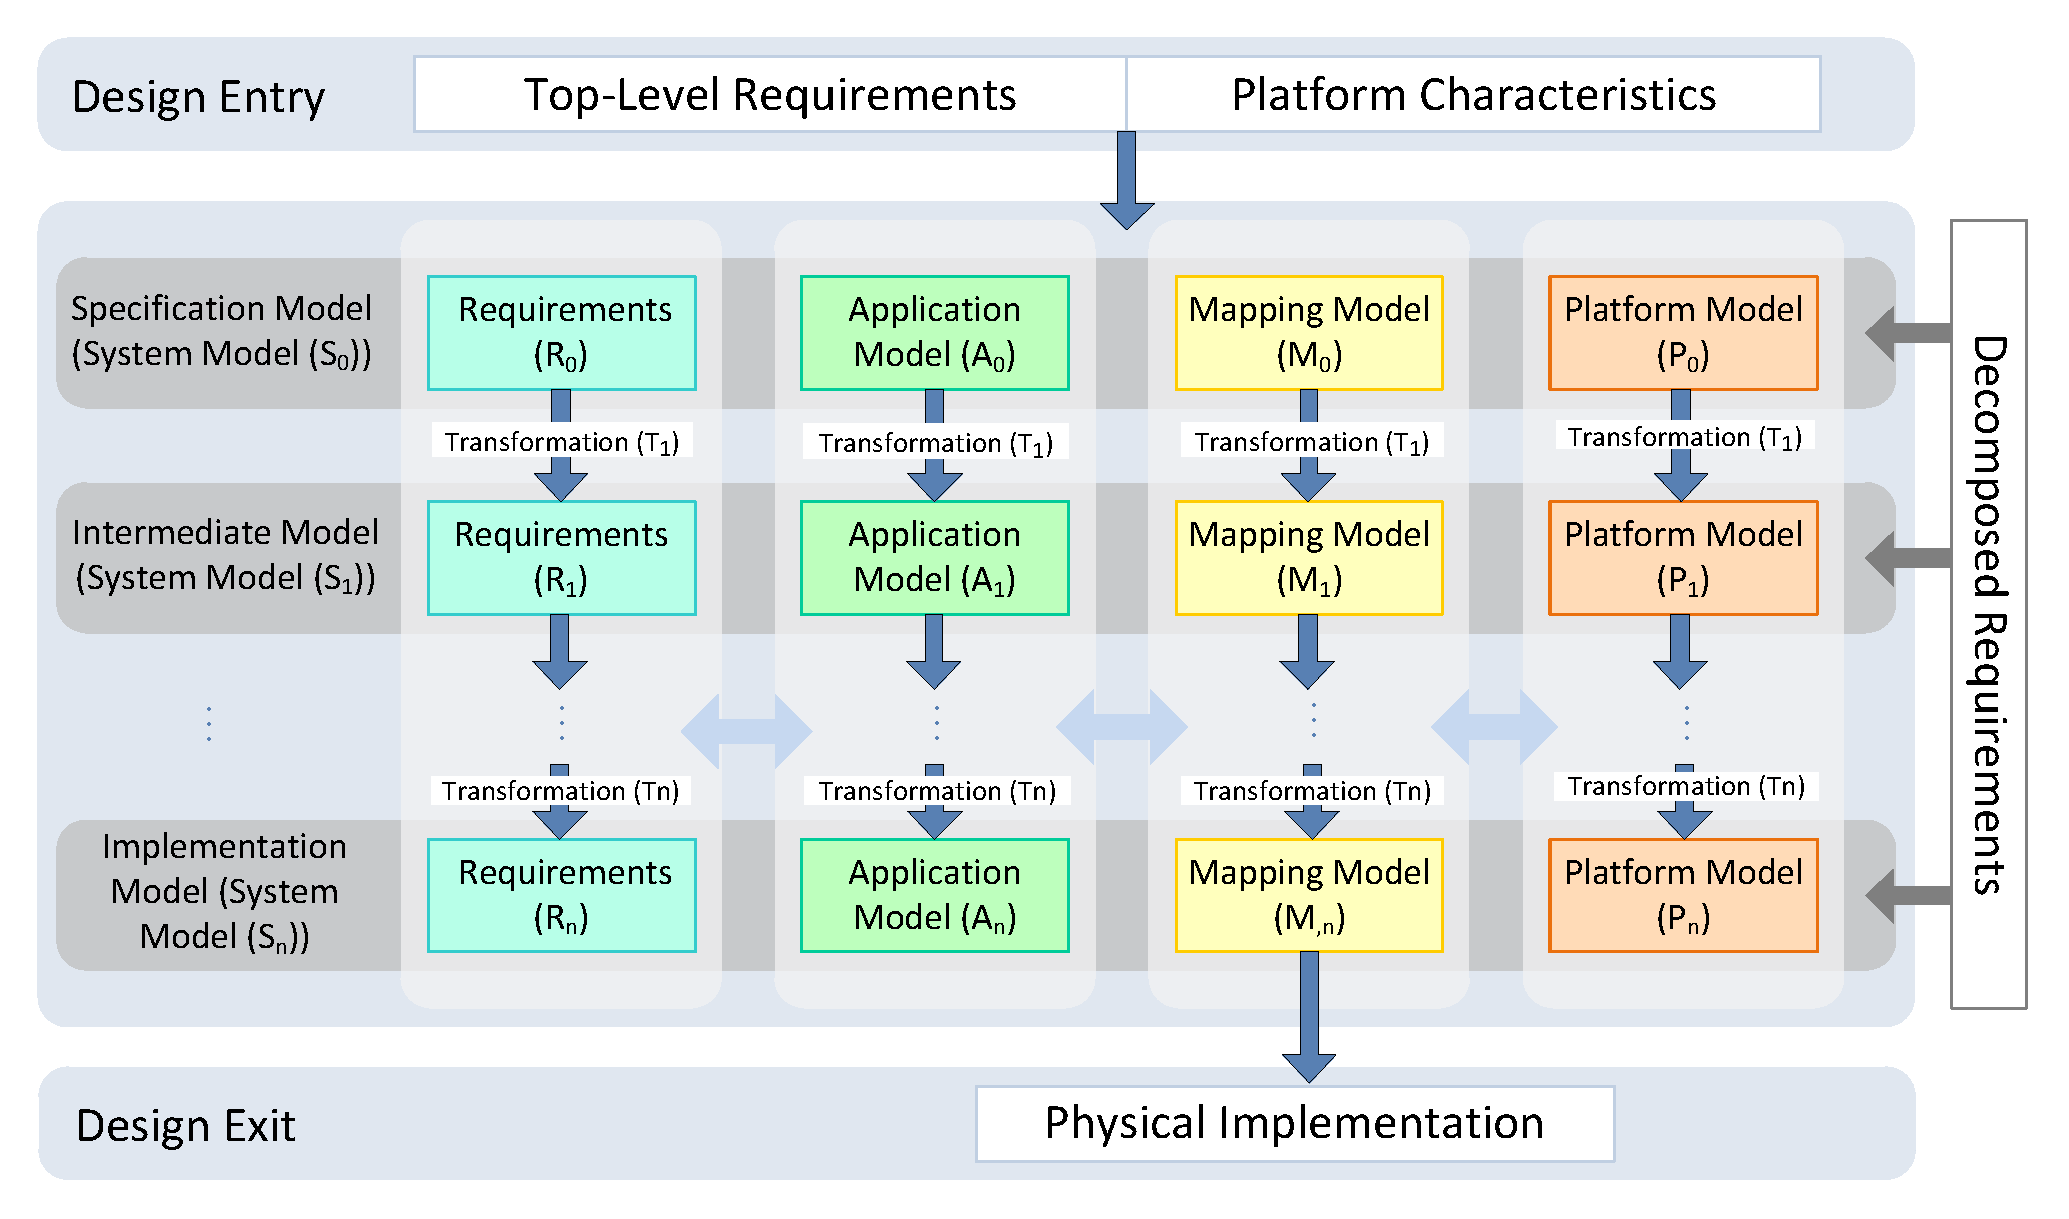
\includegraphics[width=\columnwidth]{figs-src/system-model.pdf}
	\caption{System model transformation.}
	\label{sequence}
\end{figure}

The system design process consists of a sequence of transformations, i.e., $\Gamma = \left \{T_0, T_1, ... , T_n \right\}$, with different granularity levels (Figure \ref{sequence}). At the higher abstraction levels, transformations are usually coarse grain and have been proved to have major effects on  the physical implementation \cite{kahng2009orion}. The transformation process continues until the model contains sufficient information for the synthesis to a target platform.   

In this transformation-based system design approach, a \textit{system model} $S$ is considered to consist of \textit{requirements} $R$, an \textit{application model} $A$, a \textit{mapping model} $M$, and a \textit{platform model} $P$, i.e., $S =(R,A,M,P)$. The system model is shown in Figure~\ref{sequence} and explained in the following sections. We refer to the system model in different transformation steps as \textit{RAMP}, implying slopes that connect the specification model on the highest abstraction level to the final implementation.  The vertical arrows in Figure \ref{sequence} demonstrate potential transformations, i.e., at least one of the parts of the system model is transformed at each step. The methodology allows transformations in all parts to mix and match them after each transformation.
%Table \ref{notation} denotes  all  important  notations. 
Note, that a clear separation between the application model and the platform model is emphasized in our methodology. This feature allows the designer to continuously refine both application and platform models to identify an efficient implementation.

\subsection{Application Model}
\label{sec:application model}
In our methodology, an application is considered as a function over signals.
% Because some behavior of a system that are generally considered as side effects, e.g. writing data to a register, can be formulated by a stream of its history.
This abstraction is powerful to express systems in the domain of pure functions, which provides a sound base for formal analysis. Further, we introduce models of computation (MoCs) \cite{LeeSan1998} and parallel skeletons \cite{Cole1989a,Ski1994} to model the application. This enables to explicitly specify the temporal properties and potential parallelism of an application and makes it possible to define transformations which make effects on different aspects separately. Both MoCs and skeletons can be defined as high order functions (HOFs). Hence, a consistent syntax and semantics can be defined for transformations on MoCs, skeletons or the whole application models.
%The proposed methodology supports the application models based on a  sound formal base in form of the theory of models of computation (MoC) \cite{JanSan2005a}. More specifically, the application model should be based on:
\begin{itemize}[leftmargin=*]
	\setlength{\parskip}{1pt} 
	\setlength{\itemsep}{0pt plus 0pt}
    \item \textit{Process constructors:} Following \cite{sander2004system}, the application models are process networks in which concurrent processes communicate with each other via signals. Also, in such application models, a clean separation between computation and communication is achieved by means of the concept of process constructors. A process constructor is a HOF, which takes pure functions and values as arguments, and creates a process. The process constructor describes the communication interface of the process, while the arguments to the process constructor describe the computation of the process. This clean separation is important for our transformation-based design process, since it enables to define transformation rules for processes, which have the same process constructors, but have different arguments.
    \item \textit{Skeletons:} Data-parallel skeletons enable transformations that exploit potential parallelism \cite{Cole1989a,Ski1994}. Skeletons enable to express parallel patterns and have been used to model abstract building blocks that have a predefined implementation on a parallel machine. 
\end{itemize}

Our methodology uses skeletons in tandem with process constructors to enable the transformation of application models into efficient parallel structures for which an efficient implementation in hardware and software exists.

\subsection{Platform Model}
\label{sec:platform model}

For the platform model, we follow the typical platform-based design (PBD) frameworks and highlight the features that a framework should have to support transformational view that the methodology needs \cite{attarzadeh2014framework}, \cite{nuzzo2015platform}, \cite{hendriks2020interface}. 

The  methodology  targets \textit{predictable platforms}  with  guaranteed  performance  metrics. The platform model is  built out of a library of initial components. The components are building blocks, and therefore the platform model is a block diagram consisting of interconnected
building blocks. The library should be rich enough to model different components on the set of alternative platforms. In addition, functionality of the components, i.e., what the components do, in the component library need to be in line with the constructs to build the application model. In other words, there should be hardware and software interpretations of process constructors and processes, i.e., building blocks of the application model, with determined performance metrics in the component library. Components are characterized by parameters and control functions, and therefore can model different configurations, as well as their performance metrics. Composition rules of the components, for creating a valid platform, should be also fed into the design process. 
%The framework should provide formal notations for the mentioned characteristics to enable \textit{compositional design} and \textit{compositional verification}. 
The part of the methodology related to refining the platform model pursue the goal of instantiating the components and composing them to obtain an efficient architecture that satisfies both functional and non-functional requirements.


%Furthermore, the platform modeling framework should share the same view of characterizing components with interface models \cite{hendriks2020interface} to support \textit{compositional refinement}, i.e., to refine an interface to blocks communicating with each other that implement the given interface \cite{hendriks2020interface}. Interface models are more restricted in terms of the environment, i.e., the inputs to the component (very similar to the input assumptions in assume/guarantee contracts \cite{nuzzo2015platform}, \cite{broy2012specification}). This feature of interface models lay the foundations for compositional refinement as for each component, it describes how to use a component and how it can be composed with other components. 

\subsection{Mapping Model}
\label{sec:mapping model}

For the mapping model, we use the simple but useful design space modeling technique carried out in \cite{blickle1998system}. The application model, i.e., a process network, and the platform model, i.e., a block diagram, are represented as graphs.
As they are, by construction, bipartite \cite{diestel2010graph}, the mapping model consists of edges between them, embodying any possible mapping. This
definition implies that the application and platform models must have
a \emph{corresponding} graph represention, but need not to be graph models
themselves.

\subsection{Requirements}
\label{sec:requirements}

We distinguish between traceable and untraceable requirements. System requirements are classified to \textit{decomposed requirements} and \textit{derived requirements} \cite{johnson1998178b}, \cite{landi2011arp4754a}. Decomposed requirements are top-level requirements decomposed to more detailed ones to be assigned to different subsystems. These requirements should be traceable forward and backward and should be verified after each transformation step. The requirements tree in Figure \ref{specification} illustrates decomposed requirements. However, in a design process, there are some design decisions that previously were made by designers. These design decisions are implementation-dependent and can not be captured at the higher abstraction levels. Instead, they are captured as derived requirements at the lower levels by rule-based algorithms describing acceptable decisions. Derived requirements can not be traced, however, they are powerful levers for transformations. In other words, the designer's knowledge is injected to the design flow as derived requirements and used as guidelines to achieve an efficient implementation during the transformation phase. Examples of derived requirements are requirements on robust partitioning, validity check of incoming data, redundancy, as well as requirements on maximum power consumption, computational load, and  network capacity utilization. 

%Examples of derived requirements are the execution frequency and estimated memory space needed for each task, the size of the buffers, data types, energy rules, and safety related requirements.

%\subsection{Refinements}
%\label{sec:refinement}

%The system model $S$ in transformation step $m$ is represented by the 4-tuple $S_m: (R_{i}, A_{j}, M_{k}, P_{l})$, in which $0 \leq i,j,k,l \leq m$. The indices $i,j,k,l$ shows the last transformation step in which the corresponding element is changed. In each transformation step at least one of the elements of the 4-tuple change. i.e., $(i=m) \vee (j=m) \vee (k=m) \vee (l=m) = 1$. For example, the transformation 

%$S_{m-1} \xRightarrow{T_m} S_{m}$, in which

%$S_{m-1}: (R_{m-1}, A_{m-1}, M_{m-1}, P_{m-1})$

%$S_{m}: (R_{m-1}, A_{m}, M_{m}, P_{m-1})$\\
%shows that during transformation step $m$ only the application model $A$ and the mapping model $M$ are refined. As a practical example, if the target platform is given from the beginning of the design process, $\forall m: P_{m} =~P_{0}$.

 

%%% Local Variables:
%%% mode: latex
%%% TeX-master: "../paper"
%%% End: